\documentclass{beamer}

\usepackage[czech]{babel}
\usepackage[utf8]{inputenc}
\usepackage{multicol}
\usepackage[backend=bibtex, style=iso-numeric, alldates=iso]{biblatex}

\usetheme{Madrid}
\definecolor{UBCblue}{rgb}{0, 0.698, 0.674}
\usecolortheme[named=UBCblue]{structure}

\title[Semestrální práce]{Vyhledávání K nejbližších sousedů na základě filtru}
\subtitle{Search K nearest neighbors based on a filter}
\author[Bc. Jan Jedlička, JED0050]{Bc. Jan Jedlička \\ {\footnotesize Vedoucí: Doc. Ing. Radim Bača, Ph.D.}}
\institute[]{FEI, VŠB-TUO}
\date{2022}

\titlegraphic{
\includegraphics[scale=0.2]{figures/vsb logo.jpg}}

\addbibresource{citace.bib}

\begin{document}
	
	\frame{\titlepage}
	
	\begin{frame}
		\frametitle{Úvod}
		
		\begin{itemize}
			\item Porozumění HNSW
			\item Vlastní HNSW implementace nebo zprovoznění jiné HNSW implementace
			\item Návrh a implementace rozšíření HNSW o filtr (podmínka, která stanoví, které vektory se při prohledávání vynechají)
		\end{itemize}
		
	\end{frame}

	\begin{frame}
		\frametitle{KNN}
		
		\begin{itemize}
			\item Vyhledávání K nejbližších sousedů od dotazu Q v n dimenzionálním prostoru
			\item Vzdálenost mezi body v prostoru definována metrikou (Euklidova, Hammingova, Minkowského atd.)
			\item Přibližné vyhledávání (ANN)
			\item Porovnávání vektorizovaných dat, hledání shluků, podobných vlastností (například vyhledávání sémanticky podobných dokumentů)
		\end{itemize}
		
	\end{frame}

	\begin{frame}
		\frametitle{KNN}
		\begin{figure}
			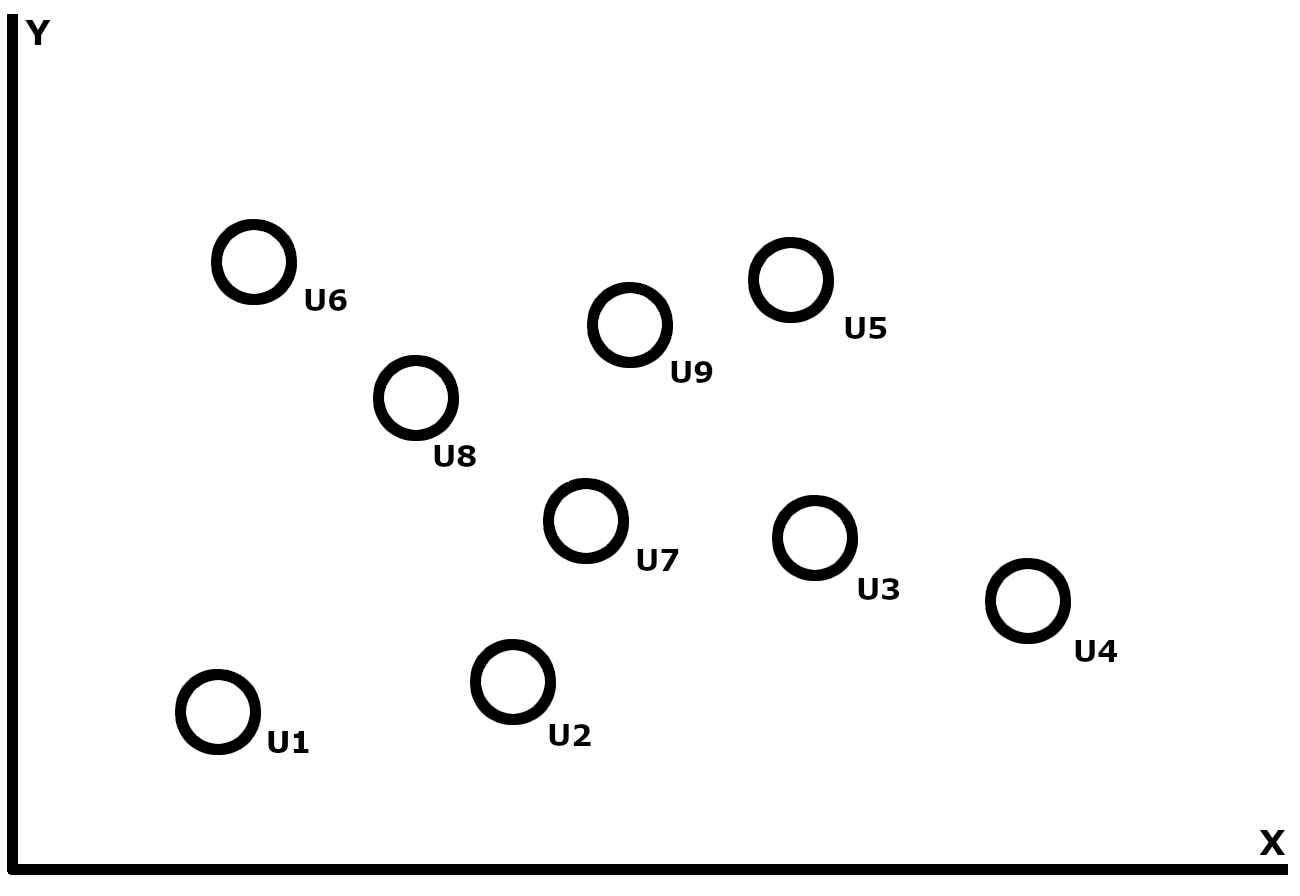
\includegraphics[scale=0.2]{figures/KNN_b1.jpg}
		\end{figure}
	\end{frame}
	
	\begin{frame}
		\frametitle{KNN}
		\begin{figure}
			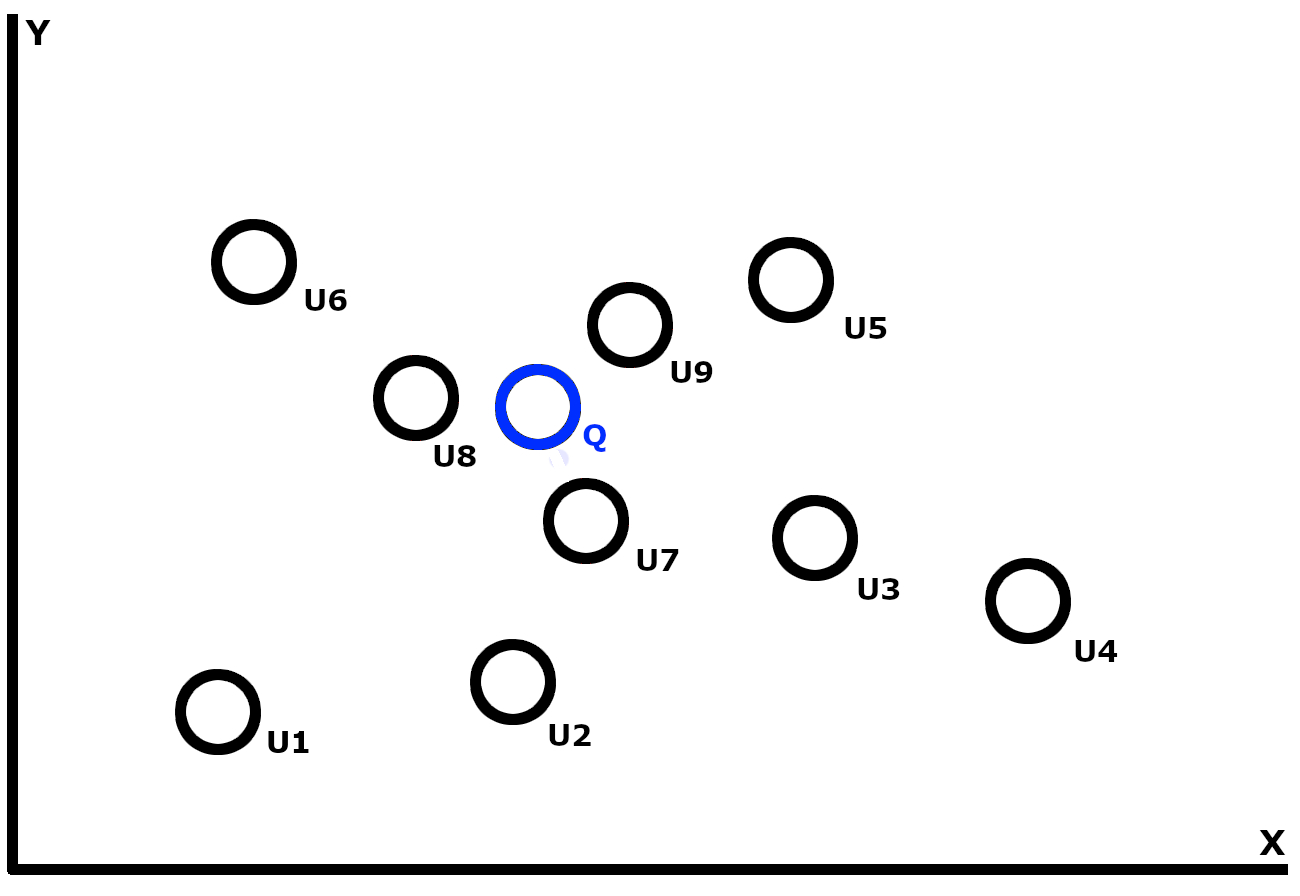
\includegraphics[scale=0.2]{figures/KNN_b2.jpg}
		\end{figure}
	\end{frame}

	\begin{frame}
		\frametitle{KNN}
		\begin{figure}
			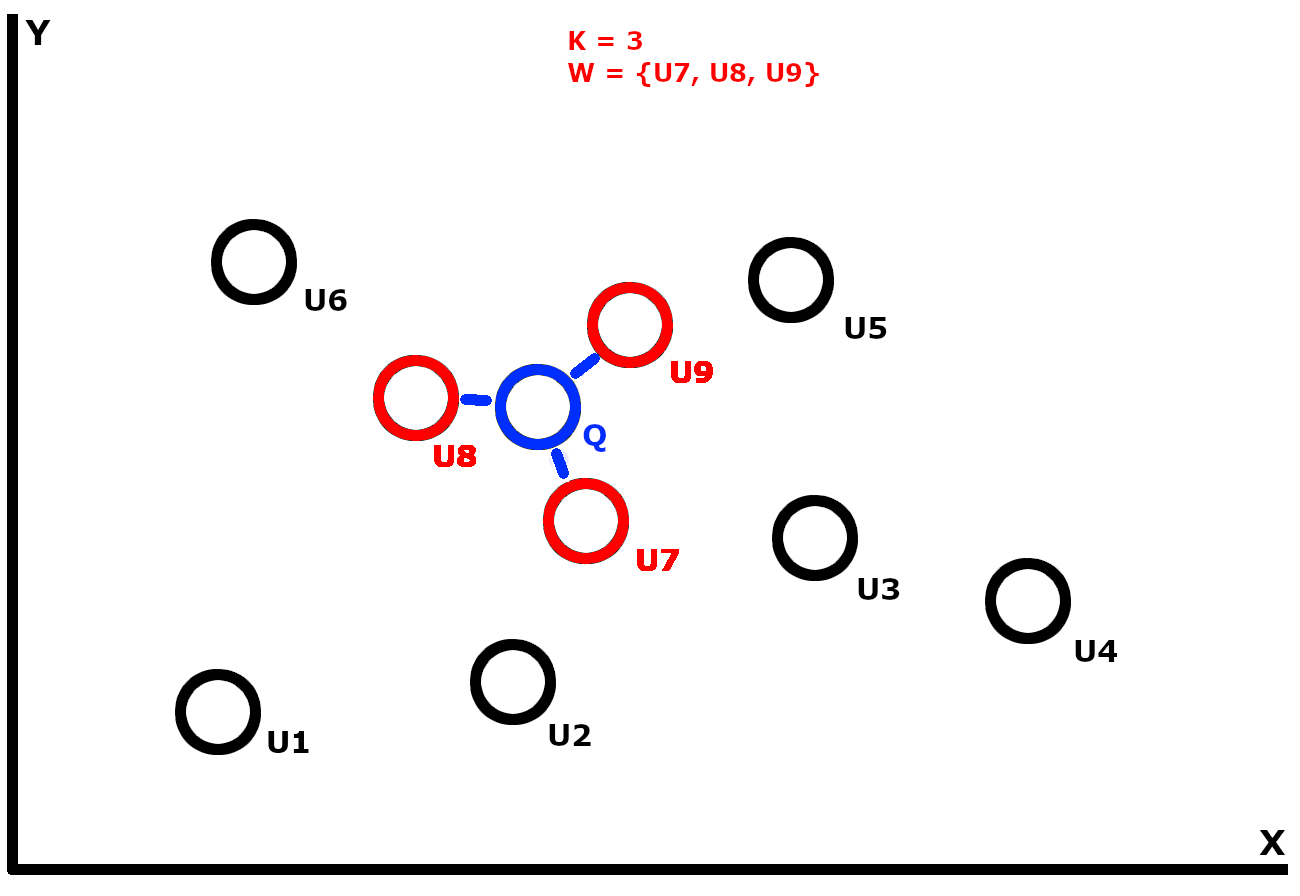
\includegraphics[scale=0.2]{figures/KNN_b3.jpg}
		\end{figure}
	\end{frame}

	\begin{frame}
		\frametitle{HNSW}
		
		\begin{itemize}
			\item Hierarchical Navigable Small Worlds
			\item Řešení KNN problému, přibližné vyhledávání s využitím vícevrstvých grafů
			\item Výsledek poskytován s určitou přesností zvanou Recall
			\item Přesnost se dá zvýšit navýšením parametru Ef, stejně tak poroste ale i čas vykonání dotazu
		\end{itemize}
		
	\end{frame}

	\begin{frame}
		\frametitle{HNSW}
		
			\begin{figure}
			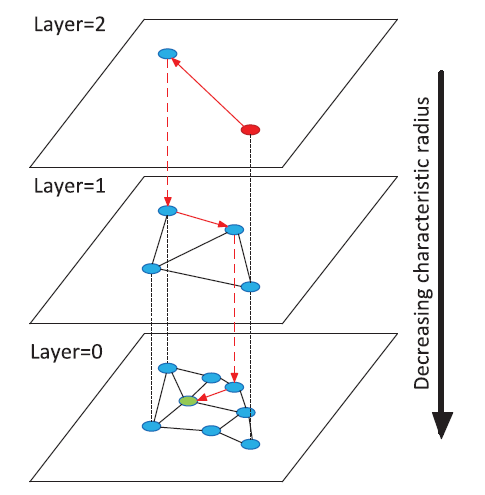
\includegraphics[scale=0.4]{figures/hnsw_layers.png}
			\caption{Vrstvy grafů v HNSW}
		\end{figure}
		
	\end{frame}

	\begin{frame}
		\frametitle{HNSW}
		
		\begin{figure}
			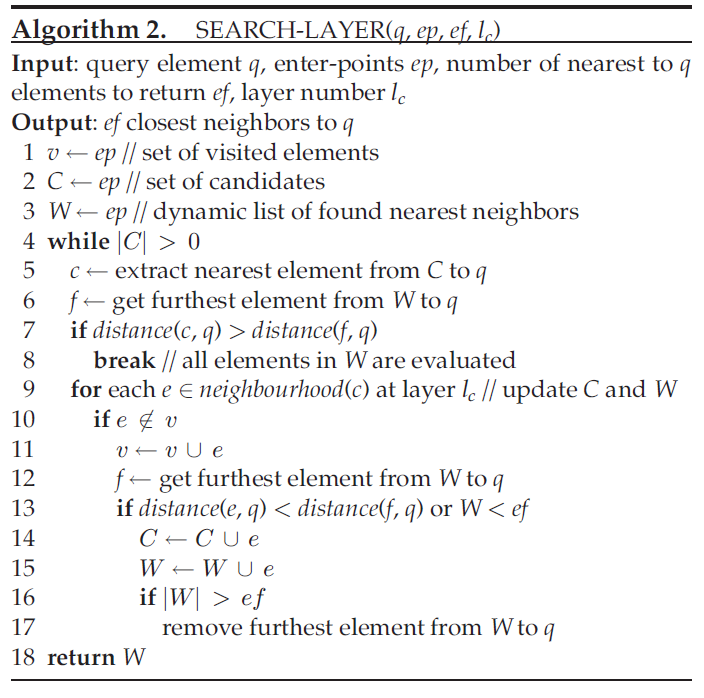
\includegraphics[scale=0.3]{figures/hnsw_search.png}
			\caption{Pseudokód HNSW Search algoritmu}
		\end{figure}
		
	\end{frame}

	\begin{frame}
		\frametitle{HNSW}
		
		\begin{figure}
			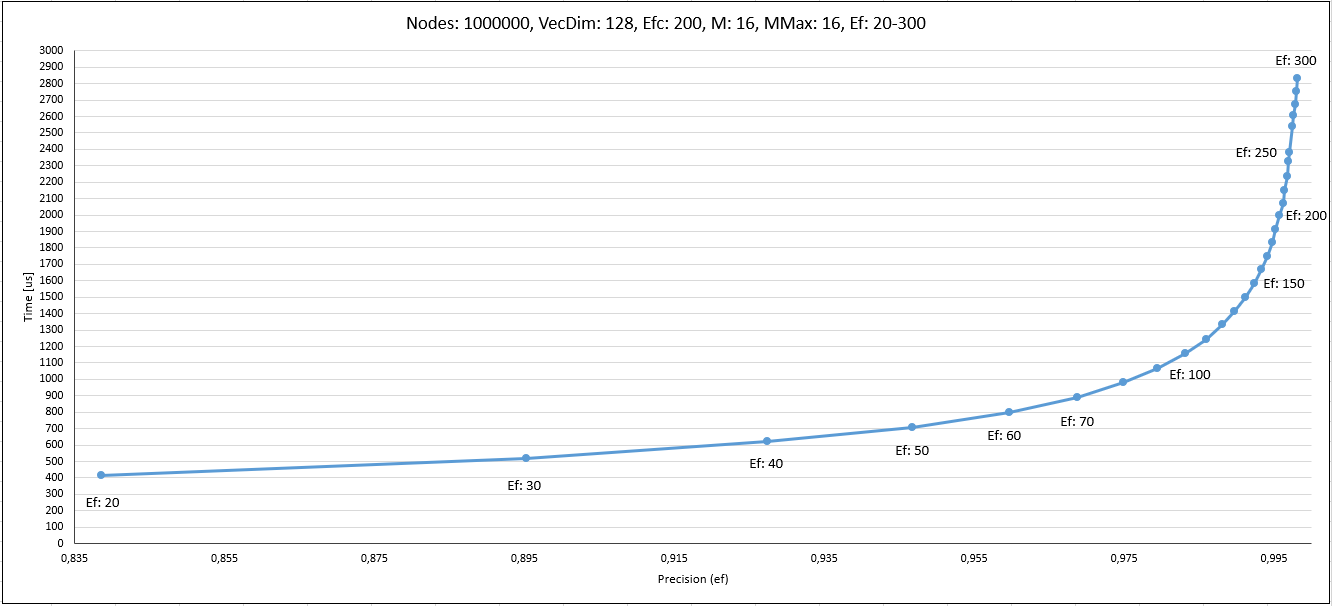
\includegraphics[scale=0.34]{figures/graf_hnsw.png}
			\caption{Graf závislosti průměrného času jednoho dotazu na přesnosti}
		\end{figure}
		
	\end{frame}

	\begin{frame}
		\frametitle{Filtr}
		
		\begin{itemize}
			\item Podmínka určující které vektory neprocházet a nevracet do výsledku
			\item Udává jakých hodnot mají nabývat jednotlivé atributy, nebo v jakých intervalech hodnot se mají nacházet
			\item Nemusíme omezovat všechny atribury
			\item Selektivita filtru $<0,1>$ udává procentuální počet uzlů z celé množiny všech uzlů, které filtr přijme
			
		\end{itemize}
		
	\end{frame}

	\begin{frame}
		\frametitle{Filtr}
		
		\begin{figure}
			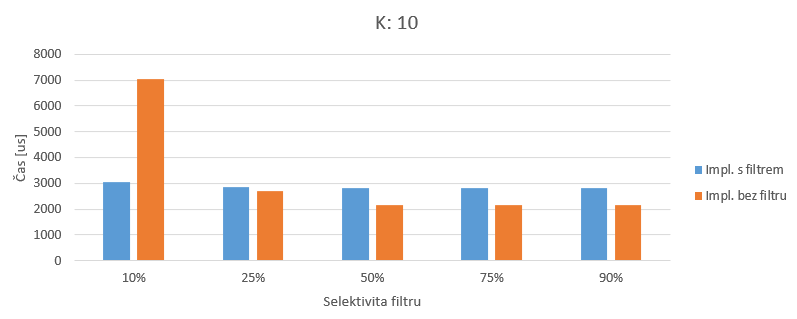
\includegraphics[scale=0.4]{figures/graf_filtr_k10.png}
		\end{figure}
	
		\begin{figure}
			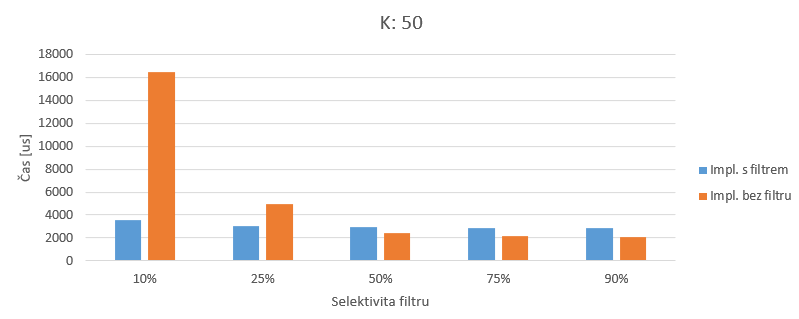
\includegraphics[scale=0.4]{figures/graf_filtr_k50.png}
		\end{figure}
		
	\end{frame}

	\begin{frame}
		\frametitle{Filtr}
		
		\begin{figure}
			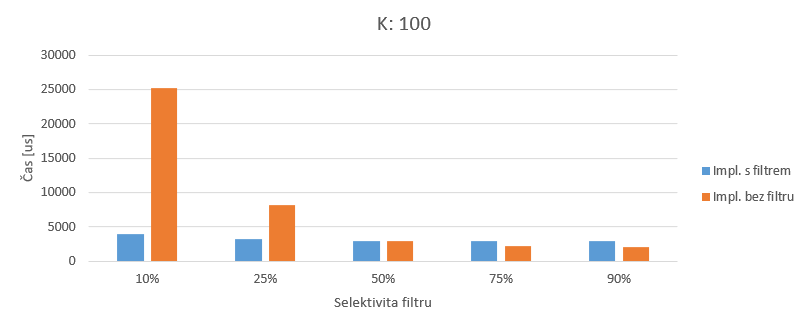
\includegraphics[scale=0.4]{figures/graf_filtr_k100.png}
		\end{figure}
		
		\begin{figure}
			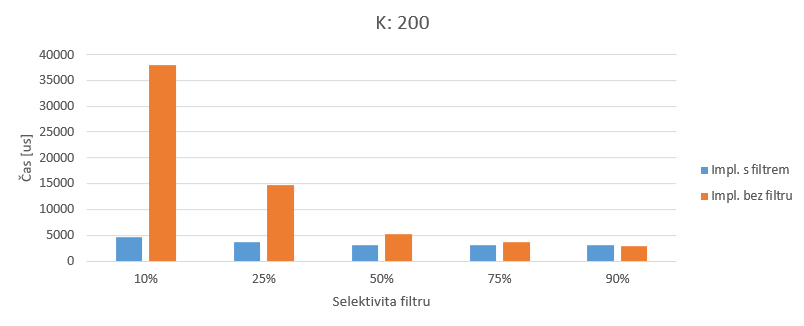
\includegraphics[scale=0.4]{figures/graf_filtr_k200.png}
		\end{figure}
		
	\end{frame}

	\begin{frame}
		\frametitle{Závěr}
		
		\begin{itemize}
			\item Splnění všech požadavků
			\item Funkční implementace původního HNSW
			\item HNSW implementace o polovinu pomalejší než reference
			\item Funkční implementace rozšířeného HNSW o filtry
		\end{itemize}
		
	\end{frame}

	\begin{frame}
		\frametitle{Poděkování}
		
		\begin{center}
			\Huge
			Děkuji za pozornost
		\end{center}
		
	\end{frame}

	\begin{frame}[noframenumbering,allowframebreaks]
		\frametitle{Citace}
		
		\nocite{*}
		
		\printbibliography
		
	\end{frame}
	
\end{document}